\begin{enumerate}[label=\thechapter.\arabic*,ref=\thechapter.\theenumi]

\item The damping ratio and undamped natural frequency of a closed loop system as
shown in the figure, are denoted as $\zeta$ and $\omega_n$, respectively. The values of $\zeta$ and $\omega_n$
are 
\begin{figure}[!ht]
\centering
\begin{center}
\includegraphics[width=\columnwidth]{2022/EE/39/figs/question.jpg}
\end{center}
%\caption{Diagram for GATE ME Question 30}
\end{figure}
\begin{enumerate}
    \item $\zeta = 0.5$ and $\omega_n = 10$ rad/s
    \item $\zeta = 0.1$ and $\omega_n = 10$ rad/s
    \item $\zeta = 0.707$ and $\omega_n = 10$ rad/s
    \item $\zeta = 0.707$ and $\omega_n = 100$ rad/s
\end{enumerate}
\hfill(GATE EE 2022)
\solution
\iffalse
\let\negmedspace\undefined
\let\negthickspace\undefined
\documentclass[journal,12pt,twocolumn]{IEEEtran}
\usepackage{cite}
\usepackage{amsmath,amssymb,amsfonts,amsthm}
\usepackage{algorithmic}
\usepackage{graphicx}
\usepackage{textcomp}
\usepackage{xcolor}
\usepackage{txfonts}
\usepackage{listings}
\usepackage{enumitem}
\usepackage{mathtools}
\usepackage{gensymb}
\usepackage{comment}
\usepackage[breaklinks=true]{hyperref}
\usepackage{tkz-euclide} 
\usepackage{listings}
\usepackage{gvv}                                        
\def\inputGnumericTable{}                                 
\usepackage[latin1]{inputenc}                                
\usepackage{color}                                            
\usepackage{array}                                            
\usepackage{longtable}                                       
\usepackage{calc}                                             
\usepackage{multirow}                                         
\usepackage{hhline}                                           
\usepackage{ifthen}                                           
\usepackage{lscape}
\usepackage{placeins}
\usepackage{xparse}


\newtheorem{theorem}{Theorem}[section]
\newtheorem{problem}{Problem}
\newtheorem{proposition}{Proposition}[section]
\newtheorem{lemma}{Lemma}[section]
\newtheorem{corollary}[theorem]{Corollary}
\newtheorem{example}{Example}[section]
\newtheorem{definition}[problem]{Definition}
\newcommand{\BEQA}{\begin{eqnarray}}
\newcommand{\EEQA}{\end{eqnarray}}
\newcommand{\define}{\stackrel{\triangle}{=}}
\theoremstyle{remark}
\newtheorem{rem}{Remark}

\graphicspath{ {./figs/} } 

\begin{document}

\bibliographystyle{IEEEtran}
\vspace{3cm}

\Large\title{GATE 2022 EE 39}
\large\author{EE23BTECH11032 - Kaustubh Parag Khachane $^{*}$% <-this % stops a space
}
\maketitle
\newpage
\bigskip

\renewcommand{\thefigure}{\theenumi}
\renewcommand{\thetable}{\theenumi}
\large\textbf{Question GATE 22 EE 39} :\\
The damping ratio and undamped natural frequency of a closed loop system as
shown in the figure, are denoted as $\zeta$ and $\omega_n$, respectively. The values of $\zeta$ and $\omega_n$
are 
\begin{figure}[!ht]
\centering
\begin{center}
\includegraphics[width=\columnwidth]{question}
\end{center}
%\caption{Diagram for GATE ME Question 30}
\end{figure}
\begin{enumerate}
    \item $\zeta = 0.5$ and $\omega_n = 10$ rad/s
    \item $\zeta = 0.1$ and $\omega_n = 10$ rad/s
    \item $\zeta = 0.707$ and $\omega_n = 10$ rad/s
    \item $\zeta = 0.707$ and $\omega_n = 100$ rad/s
\end{enumerate}
\hfill(GATE EE 2022)\\
\solution\\
\fi
\begin{table}[!ht] 
\centering
\setlength{\extrarowheight}{8pt}
\begin{tabular}{|l|l|l|}
    \hline
    \textbf{Parameter} & \textbf{Description} & \textbf{Values}\\
    \hline
     m & load of system &  \\
    \hline
     k & stiffness of system &  \\
    \hline
     $\omega_n$ & Natural frequency & $\sqrt{\frac{k}{m}}$ \\
    \hline
    $\zeta$ & Damping ratio & $\frac{c}{2m\omega_n}$ \\
    \hline
     y\brak{t} & Output of system & \\
    \hline
     x\brak{t} & Input to the system & \\
    \hline
     c & Damping coefficient & \\
    \hline
    T\brak{s} & Transfer function of system & $\frac{Y\brak{s}}{R\brak{s}}$\\
    \hline
  \end{tabular}
  \vspace{4mm}
 \caption{Parameter Table}
 \label{tab:table0_ee_22_39}
\end{table}

We will use Mason's Gain Formula to calculate the transfer function of this system. First converting the given diagram to a signal flow graph :

\begin{figure}[!ht]
\centering
\resizebox{0.5\textwidth}{!}{%
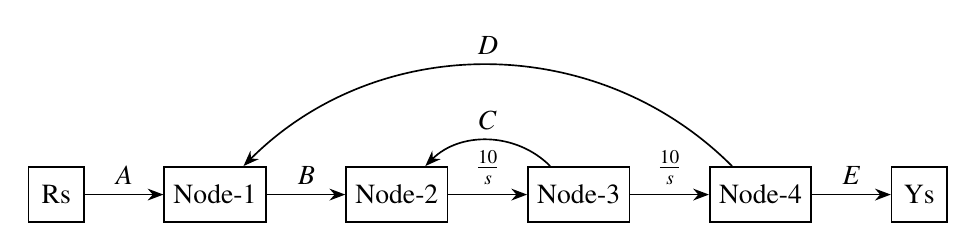
\begin{tikzpicture}[>=Stealth,auto,node distance=1cm,semithick]
  \tikzstyle{block}=[draw, fill=white, rectangle, minimum height=2em, minimum width=2em]
  
  \node [block] (input) {R\brak{s}};
  \node [block, right=of input] (filter) {Node-1};
  \node [block, right=of filter] (D) {Node-2};
  \node [block, right=of D] (E) {Node-3};
  \node [block, right=of E] (F) {Node-4};
  \node [block, right=of F] (output) {Y\brak{s}};
  
  \draw [->] (input) -- node {$A$} (filter);
  \draw [->] (filter) -- node {$B$} (D);
  \draw [->] (D) -- node {$\frac{10}{s}$} (E);
  \draw [->] (E) -- node {$\frac{10}{s}$} (F);
  \draw [->] (F) -- node {$E$} (output);
  
  % Backward loops
  \draw [->] (E) edge [bend right=45] node[above] {$C$} (D);
  \draw [->] (F) edge [bend right=45] node[above] {$D$} (filter);
\end{tikzpicture}%
}
\caption{Signal Flow Diagram}
\label{fig:your_label}
\end{figure}


Mason's Gain Formula is given by :
\begin{align}
    H\brak{s} = \sum_{i=1}^{N}\brak{\frac{P_i \Delta_i}{\Delta}} \label{eq:eq1_ee39}
\end{align}
\begin{table}[!ht] 
\centering
\setlength{\extrarowheight}{8pt}
\begin{tabular}{|l|l|}
    \hline
    \textbf{Parameter} & \textbf{Description}\\
    \hline
     N & Number of forward paths \\\hline
     L & Number of loops\\\hline
     $P_k$ & Forward path gain of $k^{th}$ path\\\hline
     $\Delta_k$ & Associated path factor \\\hline
     $\Delta$ & Determinant of the graph \\\hline
  \end{tabular}
  \vspace{4mm}
 \caption{Parameter Table - Mason's Gain Law}
 \label{tab:table1_ee_22_39}
\end{table}

\begin{table}[!ht] 
\centering
\setlength{\extrarowheight}{8pt}
\begin{tabular}{|l|l|}
    \hline
    \textbf{Parameter} & \textbf{Formula}\\
    \hline
     $\Delta$ & 1 + $\sum_{k=1}^{L}\brak{\brak{-1}^k\text{Product of gain of groups of k isolated loops}}$ \\\hline
     $\Delta_k$ & $\Delta$ part of graph that is not touching $k^{th}$ forward path \\\hline
  \end{tabular}
  \vspace{4mm}
 \caption{Formula Table - Mason's Gain Law}
 \label{tab:table2_ee_22_39}
\end{table}

This signal flow graph has only one forward path whose gain is given by :
\begin{align}
    P_1 &= \frac{10}{s} \frac{10}{s}\\
    &= \frac{100}{s^2}
\end{align}
The loop gain for loop between Node-2 and Node-3 is :
\begin{align}
    L_1 &= \frac{10}{s}\brak{-1}\\
    &= -\frac{10}{s}
\end{align}
The loop gain for loop between Node-1 and Node-4 is :
\begin{align}
    L_1 &= \frac{10}{s}\frac{10}{s}\brak{-1}\\
    &= -\frac{100}{s^2}
\end{align}
Using \tabref{tab:table2_ee_22_39}, $\Delta$ is :
\begin{align}
    \Delta &= 1 - \brak{-\frac{10}{s} - \frac{100}{s^2}}\\
    &= 1 + \frac{10}{s} + \frac{100}{s^2}
\end{align}
There are no two isolated loops available. Hence all further terms will b zero.\\
As both the loops are in contact with the only forward path,
\begin{align}
    \Delta_1 = 1
\end{align}
Using equation \eqref{eq:eq1_ee39} :
\begin{align}
    H\brak{s} &= \frac{\frac{100}{s^2}}{1 + \frac{10}{s} + \frac{100}{s^2}} \\
    &= \frac{100}{s^2 + 10s + 100}\label{eq:eq2_ee39}
\end{align}
Referring to \tabref{tab:table0_ee_22_39}, the general equation of the damping system is second order and can be written as :
\begin{align}
    m\ddot{y}(t) + c\dot{y}(t) + ky(t) = x(t)
\end{align}
Take the Laplace transform and solve for $\frac{Y\brak{s}}{X\brak{s}}$ :
\begin{align}
    \frac{Y\brak{s}}{X\brak{s}} &= \frac{\omega_n^2}{s^2 + 2\zeta\omega_n s + \omega_n^2}\\
\implies H\brak{s} &= \frac{\omega_n^2}{s^2 + 2\zeta\omega_n s + \omega_n^2} \label{eq:eq3_ee39}
\end{align}
Comparing equations \eqref{eq:eq2_ee39} and \eqref{eq:eq3_ee39} ,
\begin{align}
    \omega_n ^2 &= 100\\
    \implies \omega_n &= 10 \text{ rad/s} \label{eq:eq4_ee39}\\
    2\zeta \omega_n &= 10\\
    \implies \zeta &= 0.5
\end{align}
\begin{figure}[!ht]
\centering
\begin{center}
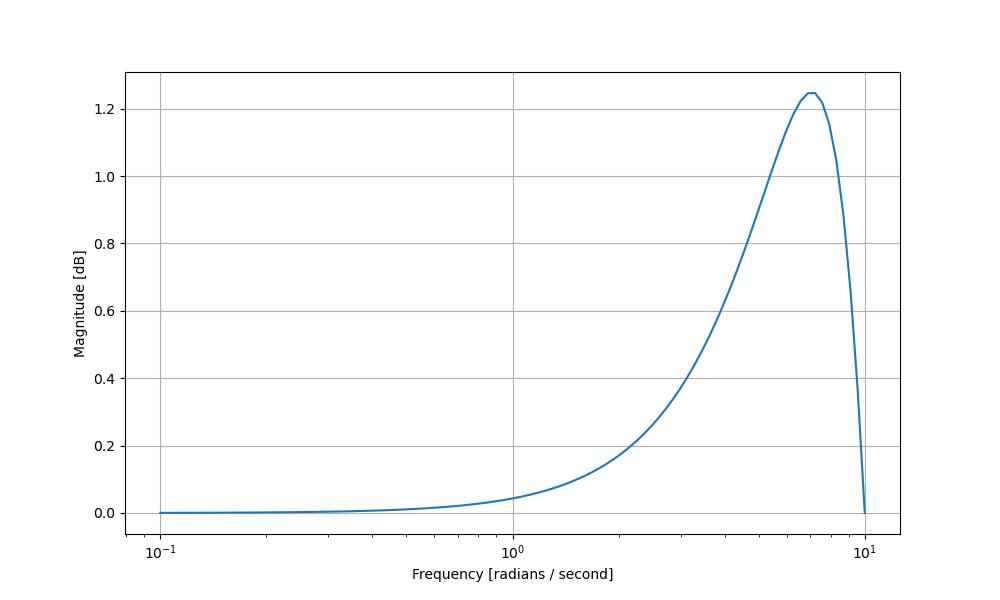
\includegraphics[width=\columnwidth]{2022/EE/39/figs/Figure_1.jpg}
\end{center}
\caption{Magnitude plot}
\end{figure}
\begin{figure}[!ht]
\centering
\begin{center}
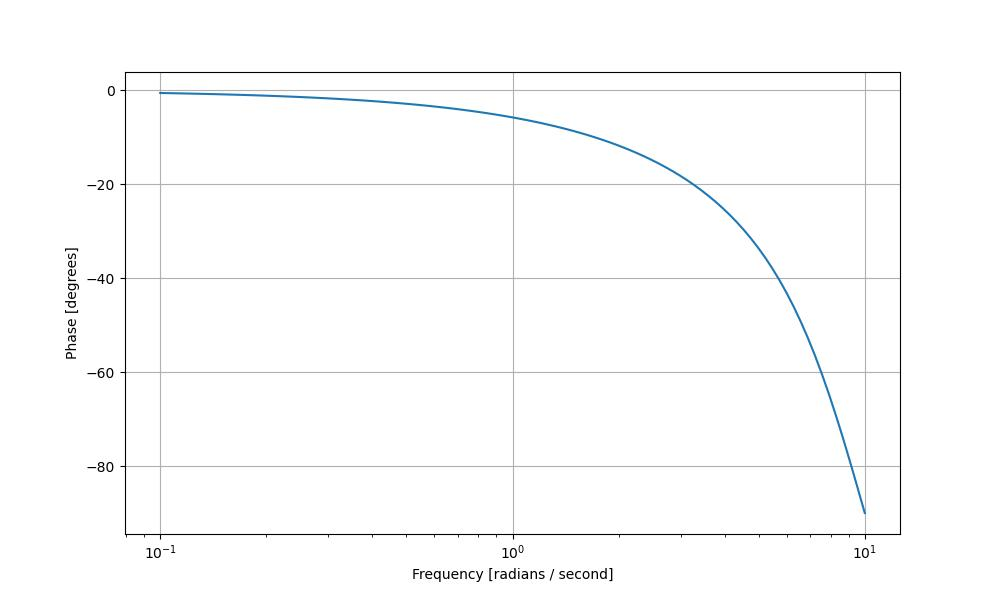
\includegraphics[width=\columnwidth]{2022/EE/39/figs/Figure_2.jpg}
\end{center}
\caption{Phase plot}
\end{figure}

\newpage
\item In the block diagram shown in the figure, the transfer function $G=\frac{K}{\tau s+1}$ with $K>0$ and $\tau>0$. The maximum value of $K$ below which the system remains stable is \rule{1cm}{0.15mm}(rounded off to two decimal places) \hfill (GATE CH 2022) 
\begin{figure}[htbp] 
\includegraphics[width=\columnwidth]{2022/CH/58/figs/question.jpg} 
\end{figure}\\ 
\solution 
\input{2022/CH/58/ch_58.tex} 
\newpage

\item
A series RLC circuit is connected to 220 V, 50 Hz supply. For a fixed a value of R and C, the inductor L is varied to deliver the maximum current. This value 0.4A and the corresponding potential drop across the capacitor is 330 V. The value of the inductor L is ? (Rounded off to two decimal places).
\hfill{(GATE BM 2022)}\\
 \solution
 \iffalse
\let\negmedspace\undefined
\let\negthickspace\undefined
\documentclass[journal,12pt,onecolumn]{IEEEtran}
\usepackage{cite}
\usepackage{amsmath,amssymb,amsfonts,amsthm}
\usepackage{algorithmic}
\usepackage{graphicx}
\usepackage{textcomp}
\usepackage{xcolor}
\usepackage{txfonts}
\usepackage{listings}
\usepackage{enumitem}
\usepackage{circuitikz}
\usepackage{mathtools}
\usepackage{gensymb}
\usepackage{comment}
\usepackage[breaklinks=true]{hyperref}
\usepackage{tkz-euclide} 
\usepackage{listings}
\usepackage{gvv}    
\usepackage{enumitem}
\usepackage{amsmath}
\def\inputGnumericTable{}                                 
\usepackage[latin1]{inputenc}                                
\usepackage{color}                                            
\usepackage{array}                                            
\usepackage{longtable}                                       
\usepackage{calc}                                             
\usepackage{multirow}                                         
\usepackage{hhline}                                           
\usepackage{ifthen}                                           
\usepackage{lscape}
\usepackage{tabularx}

\newtheorem{theorem}{Theorem}[section]
\newtheorem{problem}{Problem}
\newtheorem{proposition}{Proposition}[section]
\newtheorem{lemma}{Lemma}[section]
\newtheorem{corollary}[theorem]{Corollary}
\newtheorem{example}{Example}[section]
\newtheorem{definition}[problem]{Definition}
\newcommand{\BEQA}{\begin{eqnarray}}
\newcommand{\EEQA}{\end{eqnarray}}
\newcommand{\define}{\stackrel{\triangle}{=}}
\theoremstyle{remark}
\newtheorem{rem}{Remark}
\begin{document}
\bibliographystyle{IEEEtran}
\vspace{3cm}

\title{GATE:2022 - BM 54 }
\author{EE23BTECH11025 - Anantha Krishnan $^{}$% <-this % stops a space
}
\maketitle
\bigskip



\section{question}

A series RLC circuit is connected to 220 V, 50 Hz supply. For a fixed a value of R and C, the inductor L is varied to deliver the maximum current. This value 0.4A and the corresponding potential drop across the capacitor is 330 V. The value of the inductor L is ? (Rounded off to two decimal places).
 



\textbf{Solutions :}
\fi




\begin{table}[ht!]
\centering
\begin{tabular}{ |c|c|c| } 
 \hline
Symbols & Description & Values  \\
\hline
 $V_s$ & Input voltage & 220 V and 50Hz\\
 \hline
 $\chi_L$ & Impedance across inductor & $j\omega L$\\
 \hline
 $\chi_C$ & Impedance across capacitor & $\frac{-j}{\omega C}$\\
 \hline
 $Z$& Impedance across the entire circuit & $\frac{1}{R+j\omega L +\frac{-j}{\omega C}}$\\
 \hline
\end{tabular}
\caption{Parameters, Descriptions, and Values}
\label{table:ee25-bm54-gate2022}
\end{table}






    
    \ctikzset{bipoles/thickness=1.2}
    \newcommand{\midlabelline}[3]{
   \node (midlabel) at ($ (#1)!.5!(#2) $) {#3};
   \draw[latex-] (#1) --  (midlabel);
   \draw[-latex] (midlabel) -- (#2);
}

\begin{enumerate}
\begin{center}
\begin{circuitikz}[scale=0.8]
    % Circuit
    \draw[line width=0.6]
        (1.5,5) to [sinusoidal voltage source, l_=$220V$${,}50Hz$, i=$I$] (1.5,1)
        (1.5,5) to [resistor, l_=$R$] ++(4,0) to [inductor, l_=$L$] ++(0,-4) to [capacitor, l_=$C$] +(-4,0) ;
    
    % Voltage Infos
    \midlabelline{1.5,5.5}{5.5,5.5}{$V(R)$}
    \midlabelline{6.5,5}{6.5,1}{$V(L)$}
    \midlabelline{1.5,0}{5.5,0}{$V(C)$}
    
    % Grid
    %\draw[help lines] (0,0) grid (7,6);
\end{circuitikz}
\end{center}
    \end{enumerate}
During maximum current$\quad\abs{Z}$ is minimum .
\begin{align}
I &= \frac{V_s}{Z}\\
 &= \frac{V_s}{R+\chi_{L}+\chi_{C}}\\ 
 &=\frac{V_s}{R+j\omega L+\frac{1}{j\omega C}}\label{eq:ee25-gate2-1}\\
\quad \abs{I}&={\frac{\quad \abs{V_s}}{\sqrt{R+\brak{\omega L-\frac{1}{\omega C}^2}}}}
\end{align}
Varying $L$ for maximum value of ${I}$ :
\begin{align}
\omega L = \frac{1}{\omega C} \label{eq:ee25-gate2-2}
\end{align}
Putting in $\eqref{eq:ee25-gate2-1}$:
\begin{align}
    I_{max} &= \frac{V_s}{R}
\end{align}
$I_{max}$ has same phase as $V_s$ (Assume $\angle{\phi})$.
For impedance across the capacitor :
\begin{align}
 \left.V_C\right|_{I=I_{max}}&= I_{max} \chi_C\\
-330\angle{\brak{90+\phi}} &= \brak{0.4\angle{\phi}}\chi_C\\
-330\angle{90} &= 0.4\chi_C\\
\implies \chi_C &= -825j\si{\ohm}
\end{align}
For value of Capacitor and inductor, using \eqref{eq:ee25-gate2-2} :
\begin{align}
L &= \frac{825}{100\pi}H\\
&\approx 2.63 \si{H}\\
C &= 3.858*10^{-6} \si{F}
\end{align}


    \begin{figure}[!ht]    
    \centering
\graphicspath{ {2022/BM/54/figs/} }
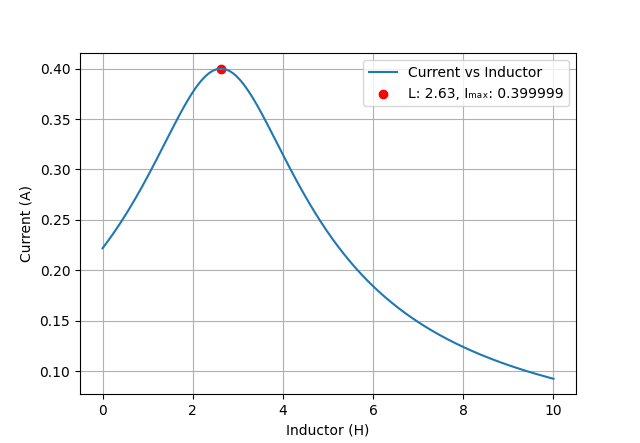
\includegraphics[width=\columnwidth]{graph_1}
\caption{ $I$ vs $L$ }
\label{graph:ee25-gate2-graph}
\end{figure}







 
 \newpage
 
 \item
 The open loop transfer function of a unity gain negative feedback system is given by $G\brak{s}= \frac{k}{s^2 +4s-5}$. The range of k for which the system is stable,is\hfill(GATE EE 2022)\\
\solution
\iffalse
\documentclass[journal,12pt,twocolumn]{IEEEtran}
\usepackage{amsmath,amssymb,amsfonts,amsthm}
\usepackage{txfonts}
\usepackage{tkz-euclide}
\usepackage{listings}
\usepackage{gvv}
\usepackage[latin1]{inputenc}
\usepackage{array}
\usepackage{pgf}
\usepackage{lmodern}
\usepackage{amsmath}
\begin{document}
\bibliographystyle{IEEEtran}

\title{GATE 2022[EE]-19}
\author{EE23BTECH11066 - Yakkala Amarnath Karthik}
\maketitle
\bibliographystyle{IEEEtran}

\textbf{Question:}\\ \\
The open loop transfer function of a unity gain negative feedback system is given by $G\brak{s}= \frac{k}{s^2 +4s-5}$. The range of k for which the system is stable,is\hfill(GATE EE 2022)\\ \\

\textbf{Solution:}\\ 
\fi
\begin{table}[ht]
  \begin{tabular}{|c|c|c|}
    \hline
    \textbf{Variable} & \textbf{Description} & \textbf{value}\\
    \hline
    $G\brak{s}$ & Open loop transfer function & $\frac{k}{s^2 +4s-5}$\\
   \hline
    1+G$\brak{s}$ & Characteristic equation & 0 \\
    \hline
    \end{tabular}
  \caption{A Table with input parameters}
  \label{tab:gate2022ee19}
\end{table}
\\
 from Table\ref{tab:gate2022ee19}\\
Characteristic equation:
\begin{align}
    1+G\brak{s}=0\\
    \implies 1+\frac{k}{s^2 +4s-5}=0\\
    \implies s^2+4s+\brak{k-5}=0
\end{align}
By routh table analysis, for a stable system:

\begin{center}
    \begin{tabular}{c|c c}
        $s^2$ & 1 & \(k-5\) \\
        $s^1$ & 4 & 0 \\
        $s^0$ & \(\frac{4\brak{k-5}-0}{4}\) & 0 \\
    \end{tabular}
\end{center}


\begin{align}
\frac{4\brak{k-5}-0}{4}>0\\
    k-5>0\\
    \implies k>5
\end{align}

\begin{figure}[ht]
    \centering
    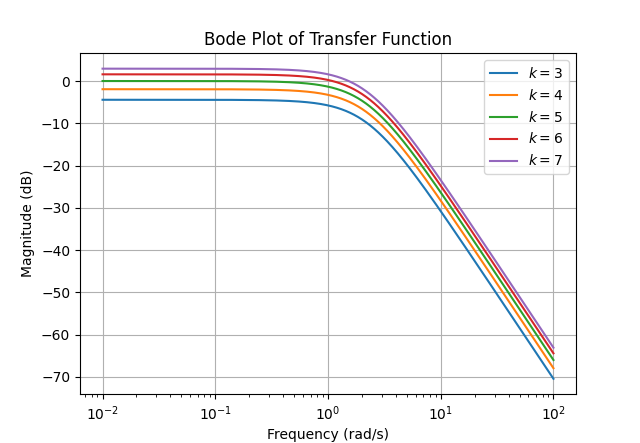
\includegraphics[width=0.45\textwidth]{2022/EE/19/figs/bodeplot.png}
    \caption{Graph showing $k<5,k=5,k>5$}
\end{figure}
For an open transfer function to be stable, its magnitude in the bode plot should be positive for some positive frequency.\\
In the below graph we can observe that the above condition satisfies for k$>$5. 
%\end{document}

\newpage
\item The signal flow graph of a system is shown. The expression for $\frac{Y\brak{s}}{X\brak{s}}$ is
\begin{figure}[h]
    \centering
    \begin{tikzpicture}
    \draw (0,0) arc (0:360:0.1);
    \draw [->] (0,0) -- (2,0);
    \draw (2.2,0) arc (0:360:0.1);
    \draw [->] (2.2,0) -- (4.2,0);
    \draw (4.4,0) arc (0:360:0.1);
    \draw [->] (4.4,0) -- (6.4,0);
    \draw (6.6,0) arc (0:360:0.1);
    \draw (-0.5,0) node[below] {$X\brak{s}$};
    \draw (1.1, 0) node[above] {$G_1\brak{s}$};
    \draw (3.3,0) node[above]  {$G_2\brak{s}$};
    \draw (5.3, 0) node[above] {$2$};
    \draw (6.9,0) node[below] {$Y\brak{s}$};
    \draw [<-](4.3,0.1) arc (0:180:1.1);
    \draw [<-] (2.1, -0.1) arc (-180:0:1.1);
    \draw  (3.2,1.3) node[above] {$G_3\brak{s}$};
    \draw (3.2,-1.2) node[below] {-1};
    \draw (2,-0.3) node[left] {$a$};
    \draw (4.3, -0.3) node[right] {$b$};
    \end{tikzpicture}
    \caption{Signal Flow Graph of the System}
    \label{fig:sfg_in-37-2022}
\end{figure}
\begin{enumerate}[label=(\alph*)]
    \item $\frac{2 G_1\brak{s} G_2\brak{s} + 2 G_1\brak{s} G_3\brak{s} }{ 1 + G_2\brak{s} + G_3\brak{s} }$
    \item $ 2 + G_1\brak{s} + G_3\brak{s} + \frac{G_2\brak{s} }{ 1 + G_2\brak{s}}$
    \item $G_1\brak{s} + G_3\brak{s} - \frac{G_2\brak{s} }{ 2 + G_2\brak{s} }$
    \item $\frac{ 2 G_1\brak{s} G_2\brak{s} + 2 G_1\brak{s} G_3\brak{s} - G_1\brak{s} }{ 1 + G_2\brak{s} + G_3\brak{s} }$
\end{enumerate}\hfill(GATE 2022 IN Question 37) \\
\solution
\iffalse
\let\negmedspace\undefined
\let\negthickspace\undefined
\documentclass[journal,12pt,twocolumn]{IEEEtran}
\usepackage{cite}
\usepackage{amsmath,amssymb,amsfonts,amsthm}
\usepackage{algorithmic}
\usepackage{graphicx}
\usepackage{textcomp}
\usepackage{xcolor}
\usepackage{txfonts}
\usepackage{listings}
\usepackage{enumitem}
\usepackage{mathtools}
\usepackage{gensymb}
\usepackage{comment}
\usepackage[breaklinks=true]{hyperref}
\usepackage{tkz-euclide} 
\usepackage{listings}
\usepackage{gvv}                                        
\def\inputGnumericTable{}                                 
\usepackage[latin1]{inputenc}                                
\usepackage{color}                                            
\usepackage{array}                                            
\usepackage{longtable}                                       
\usepackage{calc}                                             
\usepackage{multirow}                                         
\usepackage{hhline}                                           
\usepackage{ifthen}                                           
\usepackage{lscape}
\newtheorem{theorem}{Theorem}[section]
\newtheorem{problem}{Problem}
\newtheorem{proposition}{Proposition}[section]
\newtheorem{lemma}{Lemma}[section]
\newtheorem{corollary}[theorem]{Corollary}
\newtheorem{example}{Example}[section]
\newtheorem{definition}[problem]{Definition}
\newcommand{\BEQA}{\begin{eqnarray}}
\newcommand{\EEQA}{\end{eqnarray}}
\newcommand{\define}{\stackrel{\triangle}{=}}
\theoremstyle{remark}
\newtheorem{rem}{Remark}
\begin{document}

\bibliographystyle{IEEEtran}
\vspace{3cm}

\title{IN-37}
\author{EE23BTECH11063 - Vemula Siddhartha}
\maketitle
\newpage
\bigskip

\renewcommand{\thefigure}{\theenumi}
\renewcommand{\thetable}{\theenumi}
\textbf{Question}:\\
The signal flow graph of a system is shown. The expression for $\frac{Y\brak{s}}{X\brak{s}}$ is
\begin{figure}[h]
    \centering
    \begin{tikzpicture}
    \draw (0,0) arc (0:360:0.1);
    \draw [->] (0,0) -- (2,0);
    \draw (2.2,0) arc (0:360:0.1);
    \draw [->] (2.2,0) -- (4.2,0);
    \draw (4.4,0) arc (0:360:0.1);
    \draw [->] (4.4,0) -- (6.4,0);
    \draw (6.6,0) arc (0:360:0.1);
    \draw (-0.5,0) node[below] {$X\brak{s}$};
    \draw (1.1, 0) node[above] {$G_1\brak{s}$};
    \draw (3.3,0) node[above]  {$G_2\brak{s}$};
    \draw (5.3, 0) node[above] {$2$};
    \draw (6.9,0) node[below] {$Y\brak{s}$};
    \draw [<-](4.3,0.1) arc (0:180:1.1);
    \draw [<-] (2.1, -0.1) arc (-180:0:1.1);
    \draw  (3.2,1.3) node[above] {$G_3\brak{s}$};
    \draw (3.2,-1.2) node[below] {-1};
    \draw (2,-0.3) node[left] {$a$};
    \draw (4.3, -0.3) node[right] {$b$};
    \end{tikzpicture}
    \caption{Signal Flow Graph of the System}
    \label{fig:sfg_in-37-2022}
\end{figure}
\begin{enumerate}[label=(\alph*)]
    \item $\frac{2 G_1\brak{s} G_2\brak{s} + 2 G_1\brak{s} G_3\brak{s} }{ 1 + G_2\brak{s} + G_3\brak{s} }$
    \item $ 2 + G_1\brak{s} + G_3\brak{s} + \frac{G_2\brak{s} }{ 1 + G_2\brak{s}}$
    \item $G_1\brak{s} + G_3\brak{s} - \frac{G_2\brak{s} }{ 2 + G_2\brak{s} }$
    \item $\frac{ 2 G_1\brak{s} G_2\brak{s} + 2 G_1\brak{s} G_3\brak{s} - G_1\brak{s} }{ 1 + G_2\brak{s} + G_3\brak{s} }$
\end{enumerate}\hfill(GATE 2022 IN Question 37) \\
\solution
\fi
\begin{table}[h!]    
    \centering
    \begin{tabular}{|c|c|c|}
    \hline
    \textbf{Parameter} & \textbf{Description} & \textbf{Value}\\ \hline
    $Y\brak{s}$ & Output node variable &\\
    \hline
    $X\brak{s}$ & Input node variable &\\
    \hline
    $\frac{Y\brak{s}}{R\brak{s}}$ & Transfer function & ?\\
    \hline
    $P_1$ & Forward Path Gain a-b through $G_2\brak{s}$ & $ 2 G_1\brak{s} G_2\brak{s} $ \\
    \hline
    $P_2$ & Forward Path Gain a-b through $G_3\brak{s}$ & $ 2 G_1\brak{s} G_3\brak{s}$ \\
    \hline
    $\Delta_1$ & Determinant of Forward Path a-b through $G_2\brak{s}$ & $1$ \\
    \hline
    $\Delta_2$ & Determinant of Forward Path a-b through $G_3\brak{s}$ & $1$ \\
    \hline
    $L_1$ & Gain of Loop a-b through $G_2\brak{s}$ and back & $-G_2\brak{s}$ \\
    \hline
    $L_2$ & Gain of Loop a-b through $G_3\brak{s}$ and back & $-G_3\brak{s}$ \\
    \hline 
    $\Delta$ & Determinant of System & $1+G_2\brak{s}+G_3\brak{s}$ \\
    \hline
    $n$ & Number of forward paths & $2$ \\
    \hline
    \end{tabular}
    \caption{Variables Used}
  \end{table}\\
  \begin{align}
    P_1 &= \brak{G_1\brak{s}} \brak{G_2\brak{s}} \brak{2} = 2 G_1\brak{s} G_2\brak{s} \\
    P_2 &= \brak{G_1\brak{s}} \brak{G_3\brak{s}} \brak{2} = 2 G_1\brak{s} G_3\brak{s} \\
    \Delta_1 &= 1 - \brak{0} = 1 \\
    \Delta_2 &= 1 - \brak{0} = 1 \\
    L_1 &= -G_2\brak{s} \\
    L_2 &= -G_3\brak{s} \\
    \Delta &= 1 - \brak{L_1 + L_2} = 1 + G_1\brak{s} + G_2\brak{s}
  \end{align}
  From \ref{fig:sfg_in-37-2022}, Using Mason's Gain Formula,
  \begin{align}
    \frac { Y\brak{s} }{ X\brak{s} } &= \frac { \sum_{ i = 1 }^{ n } P_i \Delta_i } { \Delta } \\
    &= \frac { P_1 \Delta_1 + P_2 \Delta_2 } { \Delta } \\
    &= \frac { 2 G_1\brak{s} G_2 \brak{s} \brak{1} + 2 G_1\brak{s} G_3\brak{s} \brak{1} } { 1 + G_2\brak{s} + G_3\brak{s} } \\
    \implies \frac { Y\brak{s} }{ X\brak{s} } &= \frac { 2 G_1\brak{s} G_2\brak{s} + 2 G_1\brak{s} G_3\brak{s} } { 1 + G_2\brak{s} + G_3\brak{s} }
  \end{align}

\newpage
 \item The output of the system y\brak{t} is related to its input x\brak{t} according to the relation $y\brak{t}=x\brak{t}sin\brak{2\pi t}$.This system is 
\\\\\brak{A} Linear and time-variant
\\\brak{B} Non-Linear and time-invariant
\\\brak{C} Linear and time-invariant
\\\brak{D} Non-linear and time-variant
\\\hfill(GATE 2022 IN Question 14)
\solution
\iffalse
\let\negmedspace\undefined
\let\negthickspace\undefined
\documentclass[journal,12pt,twocolumn]{IEEEtran}
\usepackage{cite}
\usepackage{amsmath,amssymb,amsfonts,amsthm}
\usepackage{algorithmic}
\usepackage{graphicx}
\usepackage{textcomp}
\usepackage{xcolor}
\usepackage{txfonts}
\usepackage{listings}
\usepackage{enumitem}
\usepackage{mathtools}
\usepackage{gensymb}
\usepackage{comment}
\usepackage[breaklinks=true]{hyperref}
\usepackage{tkz-euclide} 
\usepackage{listings}
\usepackage{gvv}                                        
\def\inputGnumericTable{}                                 
\usepackage[latin1]{inputenc}                                
\usepackage{color}                                            
\usepackage{array}                                            
\usepackage{longtable}                                       
\usepackage{calc}                                             
\usepackage{multirow}                                         
\usepackage{hhline}                                           
\usepackage{ifthen}                                           
\usepackage{lscape}

\newtheorem{theorem}{Theorem}[section]
\newtheorem{problem}{Problem}
\newtheorem{proposition}{Proposition}[section]
\newtheorem{lemma}{Lemma}[section]
\newtheorem{corollary}[theorem]{Corollary}
\newtheorem{example}{Example}[section]
\newtheorem{definition}[problem]{Definition}
\newcommand{\BEQA}{\begin{eqnarray}}
\newcommand{\EEQA}{\end{eqnarray}}
\newcommand{\define}{\stackrel{\triangle}{=}}
\theoremstyle{remark}
\newtheorem{rem}{Remark}
\begin{document}

\bibliographystyle{IEEEtran}
\vspace{3cm}

\title{GATE 2022 IN 14}
\author{EE23BTECH11065 - prem sagar}
\maketitle
\newpage

\bigskip

\renewcommand{\thefigure}{\theenumi}
\renewcommand{\thetable}{\theenumi}
\textbf{Question}:
\\The output of the system y\brak{t} is related to its input x\brak{t} according to the relation $y\brak{t}=x\brak{t}sin\brak{2\pi t}$.This system is 
\renewcommand{\labelenumi}{\alph{enumi})}
\begin{enumerate}
\item Linear and time-variant
\item Non-Linear and time-invariant
\item Linear and time-invariant
\item Non-linear and time-variant
\end{enumerate}
\solution
\fi
\begin{table}[!ht]
\def\arraystretch{1.5}
   \centering
    \renewcommand\thetable{1}
      \begin{tabular}{|c|c|c|}
   \hline
   \textbf{Symbol} & \textbf{Value}& \textbf{Description} \\
   \hline
         $x\brak{t}$ & & input signal\\
        \hline
        $y\brak{t}$ &$x\brak{t}sin\brak{2\pi t}$  & output signal\\
        \hline
        $\tau$ &   & Time delay\\
        \hline
\end{tabular}

    \caption{input parameters}
    \label{tab:IN 14}
 \end{table}
\\ From \tabref{tab:IN 14}
\\\begin{align}
y_1\brak{t}&\leftrightarrow x_1\brak{t}
\\y_2\brak{t}&\leftrightarrow x_2\brak{t}
\\ay_1\brak{t}+by_2\brak{t}&\leftrightarrow ax_1\brak{t}+bx_2\brak{t}
\\ay_1\brak{t}+by_2\brak{t}&=\brak{ax_1\brak{t}+bx_2\brak{t}}sin\brak{2\pi t}
\end{align}
\\$\therefore$ satisfies principle of superposition
\begin{align}
ky\brak{t}&\leftrightarrow kx\brak{t}
\\ky\brak{t}&=k\brak{x\brak{t}sin\brak{2\pi t}}
\end{align}
\\$\therefore$ satisfies principle of homogenity
\\$\therefore$ it is linear
\\\\Delay in input x\brak{t}:
\begin{align}
y_1\brak{t}&=x\brak{t-\tau}sin\brak{2\pi t}
\end{align}
\\\\Delay in output y\brak{t}:
\begin{align}
y\brak{t-\tau}&=x\brak{t-\tau}sin\brak{2\pi\brak{t-\tau}}
\\y_2\brak{t}&=x\brak{t-\tau}sin\brak{2\pi\brak{t-\tau}}
\\y_1\brak{t}&\neq y_2\brak{t}
\end{align}
\\$\therefore$ it is time variant
\\$\therefore$ \brak{A} linear and time variant 
%\end{document}

\newpage
\item Two linear time-invariant systems with transfer functions 
    \begin{align*}
    G_{1}\brak{s} = \frac{10}{s^{2} + s + 1} 
    \end{align*}
    and
    \begin{align*}
    G_{2}\brak{s} = \frac{10}{s^{2}+s\sqrt{10} +10}
    \end{align*}
    have unit step responses $y_{1}\brak{t}$ and $y_{2}\brak{t}$, respectively. Which of the following statements is/are true?
    \begin{enumerate}
    \item $y_{1}\brak{t}$ and $y_{2}\brak{t}$ have the same percentage peak overshoot.\\
    \item $y_{1}\brak{t}$ and $y_{2}\brak{t}$ have the same steady state values.\\
    \item $y_{1}\brak{t}$ and $y_{2}\brak{t}$ have the same damped frequency of oscillation.\\
    \item $y_{1}\brak{t}$ and $y_{2}\brak{t}$ have the same $2\%$ settling time.\\
    \end{enumerate}
    \hfill(GATE 2022 EC Q50)\\
    \solution
    \iffalse
\documentclass[journal,12pt,onecolumn]{IEEEtran}
\usepackage{cite}
\usepackage{amsmath,amssymb,amsfonts,amsthm}
\usepackage{algorithmic}
\usepackage{graphicx}
\usepackage{textcomp}
\usepackage{xcolor}
\usepackage{txfonts}
\usepackage{listings}
\usepackage{enumitem}
\usepackage{mathtools}
\usepackage{gensymb}
\usepackage{comment}
\usepackage[breaklinks=true]{hyperref}
\usepackage{tkz-euclide}
\usepackage{listings}
\usepackage{gvv}
\def\inputGnumericTable{}
\usepackage[latin1]{inputenc}
\usepackage{color}
\usepackage{array}
\usepackage{longtable}
\usepackage{calc}
\usepackage{multirow}
\usepackage{hhline}
\usepackage{ifthen}
\usepackage{lscape}

\newtheorem{theorem}{Theorem}[section]
\newtheorem{problem}{Problem}
\newtheorem{proposition}{Proposition}[section]
\newtheorem{lemma}{Lemma}[section]
\newtheorem{corollary}[theorem]{Corollary}
\newtheorem{example}{Example}[section]
\newtheorem{definition}[problem]{Definition}
\newcommand{\BEQA}{\begin{eqnarray}}
    \newcommand{\EEQA}{\end{eqnarray}}
\newcommand{\define}{\stackrel{\triangle}{=}}
\theoremstyle{remark}
\newtheorem{rem}{Remark}

\begin{document}
    
    \bibliographystyle{IEEEtran}
    \vspace{3cm}
    
    \title{Gate 2022 EC Q50}
    \author{EE23BTECH11212 - Manugunta Meghana Sai$^{*}$% <-this % stops a space
    }
    \maketitle
    \bigskip
    
    \renewcommand{\thefigure}{\theenumi}
    \renewcommand{\thetable}{\theenumi}
    
    \vspace{3cm}
    \textbf{Gate 2022 EC Q50} 
    
    Two linear time-invariant systems with transfer functions 
    \begin{align*}
    G_{1}\brak{s} = \frac{10}{s^{2} + s + 1} 
    \end{align*}
    and
    \begin{align*}
    G_{2}\brak{s} = \frac{10}{s^{2}+s\sqrt{10} +10}
    \end{align*}
    have unit step responses $y_{1}\brak{t}$ and $y_{2}\brak{t}$, respectively. Which of the following statements is/are true?
    \begin{enumerate}
    \item $y_{1}\brak{t}$ and $y_{2}\brak{t}$ have the same percentage peak overshoot.\\
    \item $y_{1}\brak{t}$ and $y_{2}\brak{t}$ have the same steady state values.\\
    \item $y_{1}\brak{t}$ and $y_{2}\brak{t}$ have the same damped frequency of oscillation.\\
    \item $y_{1}\brak{t}$ and $y_{2}\brak{t}$ have the same $2\%$ settling time.\\
    \end{enumerate}
    \solution
    \fi
    \begin{table}[h!]
 	\centering
 	\resizebox{6 cm}{!}{
 		\begin{tabular}{|c|c|c|}
	\hline
	\textbf{Parameter} &  \textbf{Description} & \textbf{value}\\[6pt]
	\hline
	$X_{1}\brak{s}$ & input & $\frac{1}{s}$ \\[6pt]
	\hline
	$X_{2}\brak{s}$ & input & $\frac{1}{s}$ \\[6pt]
	\hline
	$G_{1}\brak{s}$ & transfer function & $\frac{10}{s^{2} + s + 1} $ \\[6pt]
	\hline
	$G_{2}\brak{s}$ & transfer function & $\frac{10}{s^{2}+s\sqrt{10} +10} $ \\[6pt]
	\hline
	$y_{1}\brak{t}$ & unit step response & $-$\\[6pt]
	\hline
	$y_{2}\brak{t}$ & unit step response & $-$\\[6pt]
	\hline
	$\omega_{n}$ & natural frequency & $-$\\[6pt]
	\hline
	$\zeta$ & damping ratio & $-$\\[6pt]
	\hline 
	
\end{tabular}

 	}
 	\caption{Given Parameters}
 	\label{tab:msmECgate50tab1}
     \end{table} 
    The general second-order transfer function is given by:
    \begin{align}
    G\brak{s} = \frac{\omega_n^2}{s^2 + 2\zeta\omega_n s + \omega_n^2}
    \end{align}
    After comparing the coefficients of $G_{1}\brak{s}$ and $G_{2}\brak{s}$,
    \begin{table}[h!]
 	\centering
 	\resizebox{6 cm}{!}{
 		\begin{tabular}{|c|c|c|}
	\hline
	\textbf{Tranfer function} &  $\omega_{n}$ & $\zeta$\\[6pt]
	\hline
	$G_{1}\brak{s}$ & $1$ & $\frac{1}{2}$ \\[6pt]
	\hline
	$G_{1}\brak{s}$ & $\sqrt{10}$ & $\frac{1}{2}$ \\[6pt]
	\hline
\end{tabular}

 	}
 	\caption{Given Parameters}
 	\label{tab:msmECgate50tab2}
     \end{table} 
    as $\zeta = \frac{1}{2}$ is less than 1, the system is underdamped.
    \begin{align}
    Y\brak{s} &= X\brak{s} G\brak{s}\\
    &= \frac{1}{s} \brak{\frac{\omega_n^2}{s^2 + 2\zeta\omega_n s + \omega_n^2}}  
    \end{align}
    Applying inverse laplace transform,
    \begin{equation}
    y(t) = 1 - \frac{e^{-\zeta \omega_n t}}{1 - \zeta^2} \sin(\omega_d t + \phi)
    \label{eq:EC50msm}
    \end{equation}
    where $\omega_{d}$ is the damped frequency of oscillation.
    \begin{equation}
    \omega_{d} = \omega_{n}\sqrt{1 - {\zeta}^2}
    \label{eq:EC50msm2eq}
    \end{equation}
    The percentage peak overshoot $\brak{PO}$:
    \begin{equation}
    PO = \left( \frac{y_{\text{max}} - y_{\text{ss}}}{y_{\text{ss}}} \right) \times 100\%
    \label{eq:EC50msm1eq}
    \end{equation}
    $y_{\text{max}}$ is obtained by differentiating~\eqref{eq:EC50msm} with respect to time and equating it to zero, substituting the value in~\eqref{eq:EC50msm},
    \begin{align}
    y_{\text{max}} = 1 + \frac{1}{\sqrt{1-{\zeta}^2}}
    \end{align}
    $y_{\text{ss}}$ is obtained by final value theorem,
    \begin{align}
    y_{\text{ss}} &= \lim_{{s \to 0}} sY(s)\\
    &= \lim_{{s \to 0}} s\frac{\omega_n^2}{s^2 + 2\zeta\omega_n s + \omega_n^2} \frac{1}{s}\\
    &= 1
    \end{align} 
    Substituting the values of $y_{\text{max}}$ and $y_{\text{ss}}$ in~\eqref{eq:EC50msm1eq}, 
    \begin{align}
    PO = \frac{1}{\sqrt{1-{\zeta}^2}} \times 100\%
    \end{align}
    $y_{1}\brak{t}$ and $y_{2}\brak{t}$ have same $\zeta$, they have same percentage peak overshoot.So, option $\brak{1}$ is correct.\\
    The steady state value of $y\brak{t}$ is given by final value theorem:
    \begin{align}
    y_{1ss} &= \lim_{{s \to 0}} sY_{1}(s)\\
    &= \lim_{{s \to 0}} s \frac{10}{s^{2} + s + 1}  \frac{1}{s}\\
    &= 10\\
    y_{2ss} &= \lim_{{s \to 0}} sY_{2}(s)\\
    &= \lim_{{s \to 0}} s \frac{10}{s^{2}+s\sqrt{10} +10}  \frac{1}{s}\\
    &= 1
    \end{align} 
    as both the unit step responses have different steady state values, option $\brak{2}$ is incorrect.\\
    From~\eqref{eq:EC50msm1eq}, as $\omega_{n}$ is different for $y_{1}\brak{t}$ and $y_{2}\brak{t}$, they have different damped frequency of oscillation. Hence option $\brak{3}$ is incorrect.\\
    Settling time $T_s$:
    \begin{align}
    T_s = \frac{4}{\zeta \omega_n}
    \end{align}
    As, $\omega_{n}$ is different for $y_{1}\brak{t}$ and $y_{2}\brak{t}$, they have different $2\%$ settling time, Hence option $\brak{4}$ is incorrect.\\
    So, only option $\brak{1}$ is correct.   
%\end{document}


    \newpage
\item Consider a single-input-single-output (SISO) system with the transfer function
\begin{align*}
G_p(s) = \frac{2\brak{s+1}}{\brak{\frac{1}{2}s+1}\brak{\frac{1}{4}s+1}}
\end{align*}
where the time constants are in minutes. The system is forced by a unit step input at
time $t = 0$. The time at which the output response reaches the maximum is \rule{1cm}{0.15mm} minutes (rounded off to two decimal places). \hfill (GATE CH 2022)\\
\solution
\iffalse
\let\negmedspace\undefined
\let\negthickspace\undefined
\documentclass[journal,12pt,twocolumn]{IEEEtran}
\usepackage{cite}
\usepackage{amsmath,amssymb,amsfonts,amsthm}
\usepackage{algorithmic}
\usepackage{graphicx}
\usepackage{textcomp}
\usepackage{xcolor}
\usepackage{txfonts}
\usepackage{listings}
\usepackage{enumitem}
\usepackage{mathtools}
\usepackage{gensymb}
\usepackage{comment}
\usepackage[breaklinks=true]{hyperref}
\usepackage{tkz-euclide} 
\usepackage{listings}
\usepackage{gvv}                                        
\def\inputGnumericTable{}                                 
\usepackage[latin1]{inputenc}                                
\usepackage{color}                                            
\usepackage{array}                                            
\usepackage{longtable}                                       
\usepackage{calc}                                             
\usepackage{multirow}                                         
\usepackage{hhline}                                           
\usepackage{ifthen}                                           
\usepackage{lscape}
\newtheorem{theorem}{Theorem}[section]
\newtheorem{problem}{Problem}
\newtheorem{proposition}{Proposition}[section]
\newtheorem{lemma}{Lemma}[section]
\newtheorem{corollary}[theorem]{Corollary}
\newtheorem{example}{Example}[section]
\newtheorem{definition}[problem]{Definition}
\newcommand{\BEQA}{\begin{eqnarray}}
\newcommand{\EEQA}{\end{eqnarray}}
\newcommand{\define}{\stackrel{\triangle}{=}}
\theoremstyle{remark}
\newtheorem{rem}{Remark}
\begin{document}

\bibliographystyle{IEEEtran}
\vspace{3cm}

\title{GATE: CH - 60.2022}
\author{EE23BTECH11224 - Sri Krishna Prabhas Yadla$^{*}$% <-this % stops a space
}
\maketitle
\newpage
\bigskip

\renewcommand{\thefigure}{\arabic{figure}}
\renewcommand{\thetable}{\arabic{table}}


\vspace{3cm}
\textbf{Question:} Consider a single-input-single-output (SISO) system with the transfer function
\begin{align*}
G_p(s) = \frac{2\brak{s+1}}{\brak{\frac{1}{2}s+1}\brak{\frac{1}{4}s+1}}
\end{align*}
where the time constants are in minutes. The system is forced by a unit step input at
time $t = 0$. The time at which the output response reaches the maximum is \rule{1cm}{0.15mm} minutes (rounded off to two decimal places). \hfill (GATE CH 2022)\\
\solution
\fi
\begin{table}[htbp]
	\centering
	\def\arraystretch{1.5}
	\begin{tabular}{|c|c|c|}
\hline
\textbf{Parameters} & \textbf{Description} & \textbf{Value} \\
\hline
$y(t)$ & Output response & \\
\hline
$G_p(s)$ & Transfer function & $\frac{2\brak{s+1}}{\brak{\frac{1}{2}s+1}\brak{\frac{1}{4}s+1}}$\\
\hline
$x(t)$ & Input & $u(t)$ \\
\hline
	$X(s)$ & Laplace transform of x(t) & $\frac{1}{s}$\\
\hline
$y'(t)$ & $\frac{dy}{dt}$ &  \\
\hline
\end{tabular}

	\caption{Parameters}
	\label{tab:parameters_ch_60}
\end{table}
\begin{align}
Y(s) &= G_p(s)X(s) \\
&= \frac{16\brak{s+1}}{s\brak{s+2}\brak{s+4}}\\
&= \frac{2}{s}+\frac{4}{s+2}-\frac{6}{s+4} \\
\label{ch60_L(u)} u(t) &\system{L} \frac{1}{s} \\
\label{ch60_L(e^-at)} e^{-at} u(t) &\system{L} \frac{1}{s+a}
\end{align}
From Laplace transforms \eqref{ch60_L(u)} and \eqref{ch60_L(e^-at)}, we get
\begin{align}
y(t) &= \brak{2+4e^{-2t}-6e^{-4t}}u(t)
\end{align}
For maximum value of $y(t)$,
\begin{align}
y'(t) &= 0\\
\implies -8e^{-2t}+24e^{-4t} &= 0\\
e^{2t} &= 3\\
\implies t &= \frac{\ln{3}}{2} \\
&\approx 0.55
\end{align}
\begin{figure}[htbp]
	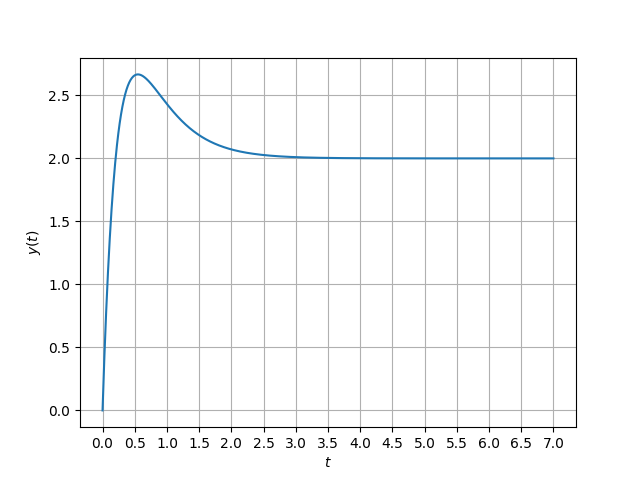
\includegraphics[width=\columnwidth]{2022/CH/60/figs/plot.png}
	\caption{Plot of $y(t)$}
	\label{fig:plot_ch60}
\end{figure}

\newpage
\item Consider the system as shown below:
\begin{center}
\begin{tikzpicture}
    % Box
    \draw (0,0) rectangle (4,2);

    % Arrow and label for x(t)
    \draw[->,>=stealth] (-1,1) -- node[above] {$x(t)$} (0,1);

    % Arrow and label for y(t)
    \draw[->,>=stealth] (4,1) -- node[above] {$y(t)$} (5,1);
\end{tikzpicture}
\end{center}


The system is described by the equation
\[ y(t) = x(e^{-t}). \]\\
The system is:
\begin{itemize}
    \item[(A)] non-linear and causal.
    \item[(B)] linear and non-causal.
    \item[(C)] non-linear and non-causal.
    \item[(D)] linear and causal.
\end{itemize}
\hfill(GATE EE 2022)\\
 \input{2022/EE/48/48.tex}
\newpage
\item The block diagrams of an ideal system and a real system with their impulse
responses are shown below. An auxiliary path is added to the delayed impulse
response in the real system.\\
\\
For a unit impulse input $\brak{x\brak{t}} = \delta \brak{t}$ to both systems, gain $\beta$ is chosen such that $y \brak{4T}$ is same for both systems. The value of $\beta$ is:
\begin{figure}[ht]
    \centering
    \includegraphics[width=\columnwidth]{2022/BM/40/figs/fig3.png}
    \label{fig: 10.5.3.128}
\end{figure}
\\
$\brak{A} e^{-3 \alpha T} \brak{1 - e^{-2 \alpha T}}$\\
\\
$\brak{B} -e^{- \alpha T} \brak{1 - e^{-3 \alpha T}}$\\
\\
$\brak{C} -e^{-3 \alpha T} \brak{1 - e^{-\alpha T}}$\\
\\
$\brak{D} e^{-2 \alpha T} \brak{1 - e^{-2 \alpha T}}$\\
\hfill(GATE BM 2022)\\
\solution
\let\negmedspace\undefined
\let\negthickspace\undefined
\documentclass[journal,12pt,twocolumn]{IEEEtran}
\usepackage{cite}
\usepackage{amsmath,amssymb,amsfonts,amsthm}
\usepackage{algorithmic}
\usepackage{graphicx}
\usepackage{textcomp}
\usepackage{xcolor}
\usepackage{txfonts}
\usepackage{listings}
\usepackage{enumitem}
\usepackage{mathtools}
\usepackage{gensymb}
\usepackage[breaklinks=true]{hyperref}
\usepackage{tkz-euclide} % loads  TikZ and tkz-base
\usepackage{listings}
\usepackage{gvv}
%
%\usepackage{setspace}
%\usepackage{gensymb}
%\doublespacing
%\singlespacing

%\usepackage{graphicx}
%\usepackage{amssymb}
%\usepackage{relsize}
%\usepackage[cmex10]{amsmath}
%\usepackage{amsthm}
%\interdisplaylinepenalty=2500
%\savesymbol{iint}
%\usepackage{txfonts}
%\restoresymbol{TXF}{iint}
%\usepackage{wasysym}
%\usepackage{amsthm}
%\usepackage{iithtlc}
%\usepackage{mathrsfs}
%\usepackage{txfonts}
%\usepackage{stfloats}
%\usepackage{bm}
%\usepackage{cite}
%\usepackage{cases}
%\usepackage{subfig}
%\usepackage{xtab}
%\usepackage{longtable}
%\usepackage{multirow}
%\usepackage{algorithm}
%\usepackage{algpseudocode}
%\usepackage{enumitem}
%\usepackage{mathtools}
%\usepackage{tikz}
%\usepackage{circuitikz}
%\usepackage{verbatim}
%\usepackage{tfrupee}
%\usepackage{stmaryrd}
%\usetkzobj{all}
%    \usepackage{color}                                            %%
%    \usepackage{array}                                            %%
%    \usepackage{longtable}                                        %%
%    \usepackage{calc}                                             %%
%    \usepackage{multirow}                                         %%
%    \usepackage{hhline}                                           %%
%    \usepackage{ifthen}                                           %%
  %optionally (for landscape tables embedded in another document): %%
%    \usepackage{lscape}     
%\usepackage{multicol}
%\usepackage{chngcntr}
%\usepackage{enumerate}

%\usepackage{wasysym}
%\documentclass[conference]{IEEEtran}
%\IEEEoverridecommandlockouts
% The preceding line is only needed to identify funding in the first footnote. If that is unneeded, please comment it out.

\newtheorem{theorem}{Theorem}[section]
\newtheorem{problem}{Problem}
\newtheorem{proposition}{Proposition}[section]
\newtheorem{lemma}{Lemma}[section]
\newtheorem{corollary}[theorem]{Corollary}
\newtheorem{example}{Example}[section]
\newtheorem{definition}[problem]{Definition}
%\newtheorem{thm}{Theorem}[section] 
%\newtheorem{defn}[thm]{Definition}
%\newtheorem{algorithm}{Algorithm}[section]
%\newtheorem{cor}{Corollary}
\newcommand{\BEQA}{\begin{eqnarray}}
\newcommand{\EEQA}{\end{eqnarray}}
\newcommand{\define}{\stackrel{\triangle}{=}}
\theoremstyle{remark}
\newtheorem{rem}{Remark}

%\bibliographystyle{ieeetr}
\begin{document}
%

\bibliographystyle{IEEEtran}


\vspace{3cm}

\title{
%	\logo{
GATE 2022 BIOMEDICAL ENGINEERING

\large{EE:1205 Signals and systems}

Indian Institute of Technology, Hyderabad
%	}
}
\author{Sai Preetam Umesh Sasankota

EE23BTECH11221
}	
%\title{
%	\logo{Matrix Analysis through Octave}{\begin{center}\includegraphics[scale=.24]{tlc}\end{center}}{}{HAMDSP}
%}


% paper title
% can use linebreaks \\ within to get better formatting as desired
%\title{Matrix Analysis through Octave}
%
%
% author names and IEEE memberships
% note positions of commas and nonbreaking spaces ( ~ ) LaTeX will not break
% a structure at a ~ so this keeps an author's name from being broken across
% two lines.
% use \thanks{} to gain access to the first footnote area
% a separate \thanks must be used for each paragraph as LaTeX2e's \thanks
% was not built to handle multiple paragraphs
%

%\author{<-this % stops a space
%\thanks{}}
%}
% note the % following the last \IEEEmembership and also \thanks - 
% these prevent an unwanted space from occurring between the last author name
% and the end of the author line. i.e., if you had this:
% 
% \author{....lastname \thanks{...} \thanks{...} }
%                     ^------------^------------^----Do not want these spaces!
%
% a space would be appended to the last name and could cause every name on that
% line to be shifted left slightly. This is one of those "LaTeX things". For
% instance, "\textbf{A} \textbf{B}" will typeset as "A B" not "AB". To get
% "AB" then you have to do: "\textbf{A}\textbf{B}"
% \thanks is no different in this regard, so shield the last } of each \thanks
% that ends a line with a % and do not let a space in before the next \thanks.
% Spaces after \IEEEmembership other than the last one are OK (and needed) as
% you are supposed to have spaces between the names. For what it is worth,
% this is a minor point as most people would not even notice if the said evil
% space somehow managed to creep in.



% The paper headers
%\markboth{Journal of \LaTeX\ Class Files,~Vol.~6, No.~1, January~2007}%
%{Shell \MakeLowercase{\textit{et al.}}: Bare Demo of IEEEtran.cls for Journals}
% The only time the second header will appear is for the odd numbered pages
% after the title page when using the twoside option.
% 
% *** Note that you probably will NOT want to include the author's ***
% *** name in the headers of peer review papers.                   ***
% You can use \ifCLASSOPTIONpeerreview for conditional compilation here if
% you desire.




% If you want to put a publisher's ID mark on the page you can do it like
% this:
%\IEEEpubid{0000--0000/00\$00.00~\copyright~2007 IEEE}
% Remember, if you use this you must call \IEEEpubidadjcol in the second
% column for its text to clear the IEEEpubid mark.



% make the title area
\maketitle

\newpage

%\tableofcontents

\bigskip

\renewcommand{\thefigure}{\theenumi}
\renewcommand{\thetable}{\theenumi}
%\renewcommand{\theequation}{\theenumi}

%\begin{abstract}
%%\boldmath
%In this letter, an algorithm for evaluating the exact analytical bit error rate  (BER)  for the piecewise linear (PL) combiner for  multiple relays is presented. Previous results were available only for upto three relays. The algorithm is unique in the sense that  the actual mathematical expressions, that are prohibitively large, need not be explicitly obtained. The diversity gain due to multiple relays is shown through plots of the analytical BER, well supported by simulations. 
%
%\end{abstract}
% IEEEtran.cls defaults to using nonbold math in the Abstract.
% This preserves the distinction between vectors and scalars. However,
% if the journal you are submitting to favors bold math in the abstract,
% then you can use LaTeX's standard command \boldmath at the very start
% of the abstract to achieve this. Many IEEE journals frown on math
% in the abstract anyway.

% Note that keywords are not normally used for peerreview papers.
%\begin{IEEEkeywords}
%Cooperative diversity, decode and forward, piecewise linear
%\end{IEEEkeywords}



% For peer review papers, you can put extra information on the cover
% page as needed:
% \ifCLASSOPTIONpeerreview
% \begin{center} \bfseries EDICS Category: 3-BBND \end{center}
% \fi
%
% For peerreview papers, this IEEEtran command inserts a page break and
% creates the second title. It will be ignored for other modes.
%\IEEEpeerreviewmaketitle	
\section{Question 40}
The block diagrams of an ideal system and a real system with their impulse
responses are shown below. An auxiliary path is added to the delayed impulse
response in the real system.\\
\\
For a unit impulse input $\brak{x\brak{t}} = \delta \brak{t}${ to both systems, gain $\beta$ is chosen such that $y \brak{4T}$ is same for both systems. The value of $\beta$ is:
\begin{figure}[ht]
    \centering
    \includegraphics[width=\columnwidth]{figs/fig3.png}
    \label{fig: 10.5.3.128}
\end{figure}
\\
$\brak{A} e^{-3 \alpha T} \brak{1 - e^{-2 \alpha T}}$\\
\\
$\brak{B} -e^{- \alpha T} \brak{1 - e^{-3 \alpha T}}$\\
\\
$\brak{C} -e^{-3 \alpha T} \brak{1 - e^{-\alpha T}}$\\
\\
$\brak{D} e^{-2 \alpha T} \brak{1 - e^{-2 \alpha T}}$\\
\section{Solution}
\begin{table}[!h]
    \centering
    \begin{tabular}{|c|c|c|}
	\hline
	\textbf{No.} & \textbf{Output} & \textbf{Function}\\[6pt]
	\hline
	$1$ & $y_I$  & $e^{- \alpha t} u\brak{t}$\\[2pt]
	\hline
	$2$ & $y_R$ & $\beta \brak{ u\brak{t} - u\brak{t-5T}} + e^{- \alpha \brak{t - T}} u\brak{t-T}$\\[2pt]
	\hline
\end{tabular} \vspace{0.5cm}
    \caption{Values} 
    \label{tab:mytable}
\end{table}
For both signals to be equal at t = 4T:\\
\begin{align}
e^{- \alpha 4T} u\brak{4T}&= \sbrak{\beta\brak{ u\brak{4T} - u\brak{-T}} + e^{- \alpha \brak{3T}} u\brak{3T}}\\
e^{- \alpha 4T} &= \beta + e^{- \alpha 3T}\\
\implies \beta &=  -e^{-3 \alpha T} \brak{1 - e^{-\alpha T}}
\end{align}
\end{document}
\newpage

\item  In a unity-gain feedback control system, the plant
$P(s) = \frac{0.001}{s\brak{2s+1}\brak{0.01s+1}}$
is controlled by a lag compensator
$C(s) = \frac{s+10}{s+0.1}$
The slope (in dB/decade) of the asymptotic Bode magnitude plot of the loop gain
at $\omega= 3 $rad/s is \_\_\_\_\_\_\_\_ (in integer)
\hfill(GATE 2022 IN)\\
\solution
\iffalse
\let\negmedspace\undefined
\let\negthickspace\undefined
\documentclass[journal,12pt,twocolumn]{IEEEtran}
\usepackage{cite}
\usepackage{amsmath,amssymb,amsfonts,amsthm}
\usepackage{algorithmic}
\usepackage{graphicx}
\usepackage{textcomp}
\usepackage{xcolor}
\usepackage{txfonts}
\usepackage{listings}
\usepackage{enumitem}
\usepackage{mathtools}
\usepackage{gensymb}
\usepackage{comment}
\usepackage[breaklinks=true]{hyperref}
\usepackage{tkz-euclide} 
\usepackage{listings}
\usepackage{gvv}                                        
\def\inputGnumericTable{}                                 
\usepackage[latin1]{inputenc}                                
\usepackage{color}                                            
\usepackage{array}                                            
\usepackage{longtable}                                       
\usepackage{calc}                                             
\usepackage{multirow}                                         
\usepackage{hhline}                                           
\usepackage{ifthen}                                           
\usepackage{lscape}
\usepackage[center]{caption} % center the captions to figure

\newtheorem{theorem}{Theorem}[section]
\newtheorem{problem}{Problem}
\newtheorem{proposition}{Proposition}[section]
\newtheorem{lemma}{Lemma}[section]
\newtheorem{corollary}[theorem]{Corollary}
\newtheorem{example}{Example}[section]
\newtheorem{definition}[problem]{Definition}
\newcommand{\BEQA}{\begin{eqnarray}}
\newcommand{\EEQA}{\end{eqnarray}}
\newcommand{\define}{\stackrel{\triangle}{=}}
\theoremstyle{remark}
\newtheorem{rem}{Remark}
\begin{document}

\newcolumntype{M}[1]{>{\centering\arraybackslash}m{#1}}
\newcolumntype{N}{@{}m{0pt}@{}}

\bibliographystyle{IEEEtran}
\vspace{3cm}

\title{GATE 2022 BM 14 Q} 
\author{ee23btech11223 - Soham Prabhakar More% <-this % stops a space
}
\maketitle
\newpage
\bigskip

\renewcommand{\thefigure}{\theenumi}
\renewcommand{\thetable}{\theenumi}

\bibliographystyle{IEEEtran}

\textbf{Question:} $x\brak{t}$ is a real continuous-time signal whose magnitude frequency response
$\abs{X\brak{j\Omega}}$ is shown below. After sampling $x\brak{t}$ at 100 $rad.s^{-1}$, the spectral point P
is down-converted to \rule{1cm}{0.15mm} $rad.s^{-1}$ in the spectrum of the sampled signal.
\hfill{(GATE 2022 BM 14 Q)}
\begin{figure}[h!]
    \renewcommand\thefigure{1}
    \centering
    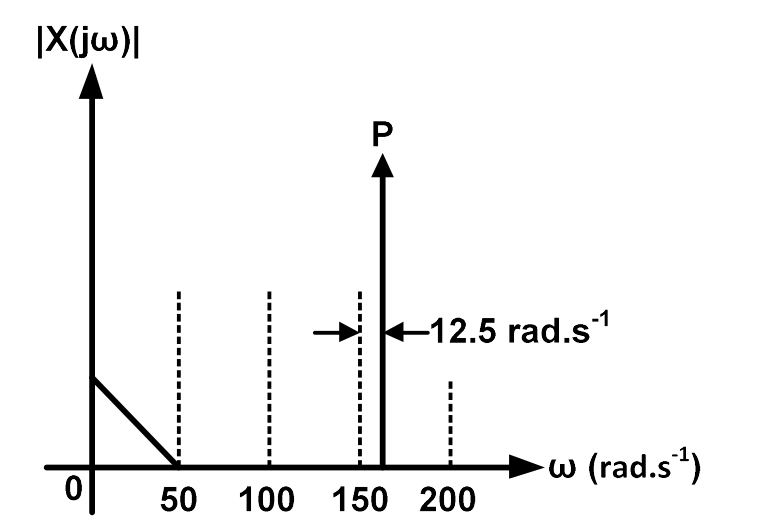
\includegraphics[width=\columnwidth]{2022/BM/14/figs/question.png}
    \caption[short]{Plot of $\abs{X\brak{j\omega}}$}
    \label{fig:2023.bm.14.img1}
\end{figure}

\solution
\fi
\begin{table}[ht]
    \renewcommand\thetable{1}
\begin{tabular}{|c|c|}
    \hline 
    \textbf{Parameter}&\textbf{Description} \\
    \hline
    $w\brak{t}$ & Sampling Function \\
    \hline
	$W\brak{j\omega}$ & Fourier Transform of $w\brak{t}$ \\
    \hline
    $x\brak{t}$ & Input Signal \\
    \hline
    $X\brak{j\omega}$ & Input Signal Frequency Spectrum \\
    \hline
    $x_s\brak{t}$ & Sampled Input Signal \\
    \hline
    $X_s\brak{j\omega}$ & Sampled Signal Frequency Spectrum \\
    \hline
\end{tabular}

\caption{Table of parameters}
\label{Table:1}


\end{table} \\
The sampling function is:
\begin{align}
    w(t) &= \sum_{k = -\infty}^{\infty}\delta\brak{t - \frac{2\pi k}{100}} \\
    W(j\omega) &= 100\sum_{k = -\infty}^{\infty}\delta\brak{j\brak{\omega - 100k}}
\end{align}
then the sampled function: 
\begin{align}
    x_s\brak{t} &= x\brak{t}w\brak{t} \\
    X_s\brak{j\omega} &= X\brak{j\omega} * W\brak{j\omega} \\
    X_s\brak{j\omega} &= \int_{-\infty}^{\infty}X\brak{j\theta}W\brak{j\brak{\omega - \theta}}d\theta \\
    X_s\brak{j\omega} &= 100\sum_{k = -\infty}^{\infty}\int_{-\infty}^{\infty}X\brak{j\theta}\delta\brak{j\brak{\omega - 100k - \theta}}d\theta \\
    X_s\brak{j\omega} &= 100\sum_{k = -\infty}^{\infty}X\brak{j\brak{\omega - 100k}} 
\end{align}
Thus, The down sampled point is at:
\begin{align}
    \omega &= \abs{162.5 - 100k}
\end{align}
where $k$ is the nearest integer to $\frac{162.5}{100}$, which is 2\\
Thus,
\begin{align}
    \omega = 37.5\,rad\,s^{-1}
\end{align}

\begin{figure}[h!]
    \renewcommand\thefigure{2}
    \centering
    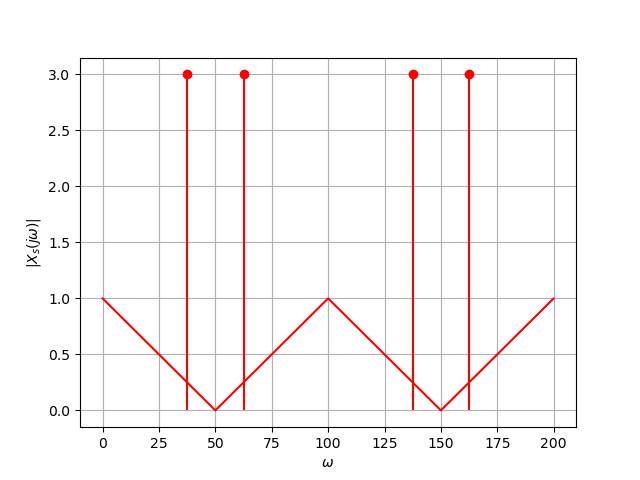
\includegraphics[width=\columnwidth]{2022/BM/14/figs/X_s.png}
    \caption[short]{Plot of $\abs{X_s\brak{j\omega}}$}
    \label{fig:2023.bm.14.img2}
\end{figure}

%\end{document}

\newpage

\item The voltage at the input of an AC-DC rectifier is given by $v\brak{t}=230\sqrt{2}\sin{\omega t}$, where $\omega=2\pi\times 50$rad/s. The input current drawn by the rectifier is given by
\begin{align*}
    i\brak{t}=10\sin\brak{\omega t-\frac{\pi}{3}}+4\sin\brak{3\omega t-\frac{\pi}{6}}+3\sin\brak{5\omega t-\frac{\pi}{3}}
\end{align*}
The power input, (rounded off to two decimal places), is\rule{1.5cm}{0.15mm}lag. \hfill(Gate 2022 EE 33Q)

\solution
\iffalse
\let\negmedspace\undefined
\let\negthickspace\undefined
\documentclass[journal,12pt,twocolumn]{IEEEtran}
\usepackage{cite}
\usepackage{amsmath,amssymb,amsfonts,amsthm}
\usepackage{algorithmic}
\usepackage{graphicx}
\usepackage{textcomp}
\usepackage{xcolor}
\usepackage{txfonts}
\usepackage{listings}
\usepackage{enumitem}
\usepackage{mathtools}
\usepackage{gensymb}
\usepackage{comment}
\usepackage[breaklinks=true]{hyperref}
\usepackage{tkz-euclide} 
\usepackage{listings}
\usepackage{gvv}                                        
\def\inputGnumericTable{}                                 
\usepackage[latin1]{inputenc}                                
\usepackage{color}                                            
\usepackage{array}                                            
\usepackage{longtable}                                       
\usepackage{calc}                                             
\usepackage{multirow}                                         
\usepackage{hhline}                                           
\usepackage{ifthen}                                           
\usepackage{lscape}
\usepackage[center]{caption} % center the captions to figure

\newtheorem{theorem}{Theorem}[section]
\newtheorem{problem}{Problem}
\newtheorem{proposition}{Proposition}[section]
\newtheorem{lemma}{Lemma}[section]
\newtheorem{corollary}[theorem]{Corollary}
\newtheorem{example}{Example}[section]
\newtheorem{definition}[problem]{Definition}
\newcommand{\BEQA}{\begin{eqnarray}}
\newcommand{\EEQA}{\end{eqnarray}}
\newcommand{\define}{\stackrel{\triangle}{=}}
\theoremstyle{remark}
\newtheorem{rem}{Remark}
\begin{document}

\newcolumntype{M}[1]{>{\centering\arraybackslash}m{#1}}
\newcolumntype{N}{@{}m{0pt}@{}}

\bibliographystyle{IEEEtran}
\vspace{3cm}

\title{GATE 2022 BM 14 Q} 
\author{ee23btech11223 - Soham Prabhakar More% <-this % stops a space
}
\maketitle
\newpage
\bigskip

\renewcommand{\thefigure}{\theenumi}
\renewcommand{\thetable}{\theenumi}

\bibliographystyle{IEEEtran}

\textbf{Question:} $x\brak{t}$ is a real continuous-time signal whose magnitude frequency response
$\abs{X\brak{j\Omega}}$ is shown below. After sampling $x\brak{t}$ at 100 $rad.s^{-1}$, the spectral point P
is down-converted to \rule{1cm}{0.15mm} $rad.s^{-1}$ in the spectrum of the sampled signal.
\hfill{(GATE 2022 BM 14 Q)}
\begin{figure}[h!]
    \renewcommand\thefigure{1}
    \centering
    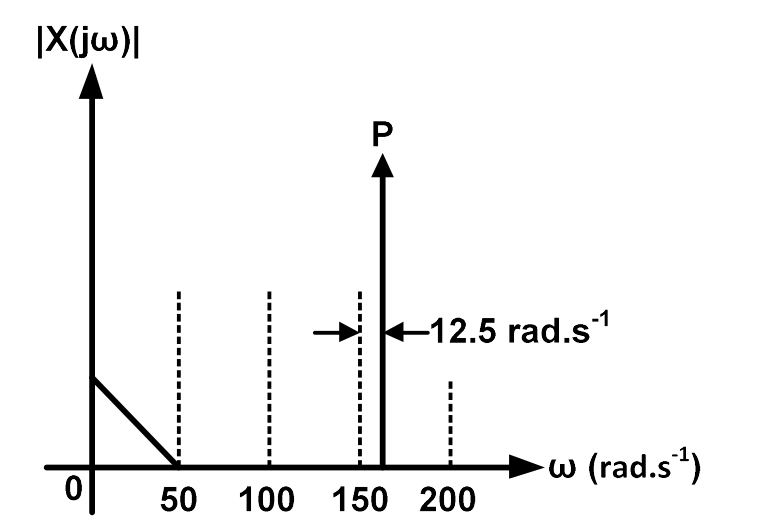
\includegraphics[width=\columnwidth]{2022/BM/14/figs/question.png}
    \caption[short]{Plot of $\abs{X\brak{j\omega}}$}
    \label{fig:2023.bm.14.img1}
\end{figure}

\solution
\fi
\begin{table}[ht]
    \renewcommand\thetable{1}
\begin{tabular}{|c|c|}
    \hline 
    \textbf{Parameter}&\textbf{Description} \\
    \hline
    $w\brak{t}$ & Sampling Function \\
    \hline
	$W\brak{j\omega}$ & Fourier Transform of $w\brak{t}$ \\
    \hline
    $x\brak{t}$ & Input Signal \\
    \hline
    $X\brak{j\omega}$ & Input Signal Frequency Spectrum \\
    \hline
    $x_s\brak{t}$ & Sampled Input Signal \\
    \hline
    $X_s\brak{j\omega}$ & Sampled Signal Frequency Spectrum \\
    \hline
\end{tabular}

\caption{Table of parameters}
\label{Table:1}


\end{table} \\
The sampling function is:
\begin{align}
    w(t) &= \sum_{k = -\infty}^{\infty}\delta\brak{t - \frac{2\pi k}{100}} \\
    W(j\omega) &= 100\sum_{k = -\infty}^{\infty}\delta\brak{j\brak{\omega - 100k}}
\end{align}
then the sampled function: 
\begin{align}
    x_s\brak{t} &= x\brak{t}w\brak{t} \\
    X_s\brak{j\omega} &= X\brak{j\omega} * W\brak{j\omega} \\
    X_s\brak{j\omega} &= \int_{-\infty}^{\infty}X\brak{j\theta}W\brak{j\brak{\omega - \theta}}d\theta \\
    X_s\brak{j\omega} &= 100\sum_{k = -\infty}^{\infty}\int_{-\infty}^{\infty}X\brak{j\theta}\delta\brak{j\brak{\omega - 100k - \theta}}d\theta \\
    X_s\brak{j\omega} &= 100\sum_{k = -\infty}^{\infty}X\brak{j\brak{\omega - 100k}} 
\end{align}
Thus, The down sampled point is at:
\begin{align}
    \omega &= \abs{162.5 - 100k}
\end{align}
where $k$ is the nearest integer to $\frac{162.5}{100}$, which is 2\\
Thus,
\begin{align}
    \omega = 37.5\,rad\,s^{-1}
\end{align}

\begin{figure}[h!]
    \renewcommand\thefigure{2}
    \centering
    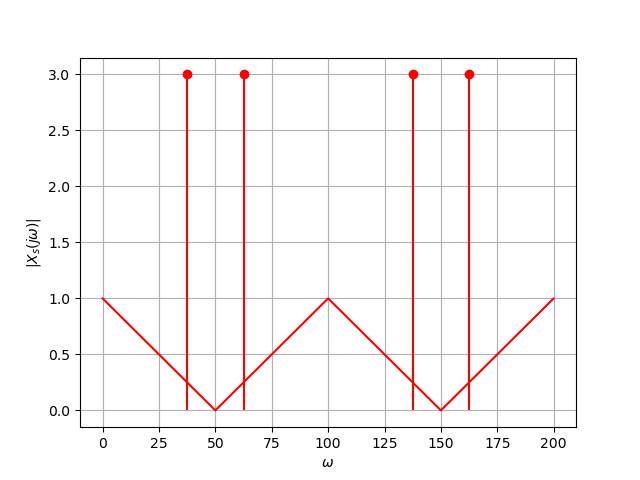
\includegraphics[width=\columnwidth]{2022/BM/14/figs/X_s.png}
    \caption[short]{Plot of $\abs{X_s\brak{j\omega}}$}
    \label{fig:2023.bm.14.img2}
\end{figure}

%\end{document}

\newpage
\item The transfer function of a system is:\\
\begin{center}
$\displaystyle \frac { \brak{s+1}\brak{s+3}}{\brak{s+5}\brak{s+7}\brak{s+9}}$\\
\end{center}
In the state-space representation of the system, the minimum number of state variables (in integer) necessary is\underline{\hspace{1cm}}.\\
\hfill(GATE IN 2022)\\
\solution\\
\iffalse
\let\negmedspace\undefined
\let\negthickspace\undefined
\documentclass[a4,12pt,onecolumn]{IEEEtran}
\usepackage{amsmath,amssymb,amsfonts,amsthm}
\usepackage{algorithmic}
\usepackage{graphicx}
\usepackage{textcomp}
\usepackage{xcolor}
\usepackage{txfonts}
\usepackage{listings}
\usepackage{enumitem}
\usepackage{mathtools}
\usepackage{gensymb}
\usepackage[breaklinks=true]{hyperref}
\usepackage{tkz-euclide}
\usepackage{listings}
\usepackage{circuitikz}
\usepackage{gvv}
\newcommand{\mybmat}[1]{\ensuremath{\begin{bmatrix}#1\end{bmatrix}}}
\begin{document}
\title{
\Huge\textbf{ GATE 2022 Assignment}\\
\Huge\textbf{EE1205} Signals and Systems\\
}
\large\author{Kurre Vinay\\EE23BTECH11036}
\maketitle
\textbf{Question:}
The transfer function of a system is:\\
\begin{center}
$\displaystyle \frac { \brak{s+1}\brak{s+3}}{\brak{s+5}\brak{s+7}\brak{s+9}}$\\
\end{center}
In the state-space representation of the system, the minimum number of state variables (in integer) necessary is\underline{\hspace{1cm}}.\\
\hfill(GATE IN 2022)\\
\solution\\
\fi
\begin{table}[ht!]
\begin{center}
\begin{tabular}{|c|c|c|}
	   \hline
	   variable&value&description\\
	   \hline
	   U\brak{s}&-&input function of the system\\
	   \hline
	   Y\brak{s}&-&output function of the system\\
	   \hline
	   H\brak{s}&$\frac { \brak{s+1}\brak{s+3}}{\brak{s+5}\brak{s+7}\brak{s+9}}$&transfer function of the system.\\
	   \hline
	   I&-&identity matrix \\
	   \hline
	   $\vec{\dot{x}}\brak{t}$ & $A\vec{x}\brak{t} + Bu\brak{t}$&derivative of State function of $ \vec{x}\brak{t}$\\
	   \hline
\end{tabular}
\caption{Table: Input Parameters}
\label{tab:1}
\end{center}
\end{table}
From \tabref{tab:1}
\begin{align}
H\brak{s}&=\frac{\brak{s+1}\brak{s+3}}{\brak{s+5}\brak{s+7}\brak{s+9}}\\
H\brak{s}&= \frac{P}{s+5} +\frac{Q}{s+7} + \frac{R}{s+9}\\
\brak{s+1}\brak{s+3}&=P\brak{s+7}\brak{s+9}+Q\brak{s+5}\brak{s+9}+R\brak{s+5}\brak{s+7} \label{eq:gate2022}
\end{align}
By solving equation \eqref{eq:gate2022} , we get\\
\begin{center}
P = 1\\
Q = -6\\
R = 6
\end{center}

\begin{align}
\implies H\brak{s}&=\frac{1}{s+5} -\frac{6}{s+7} + \frac{6}{s+9}\\
\end{align}
The state-space representation of the system is given by:
\begin{align}
\vec{\dot{x}}\brak{t} &=A\vec{x}\brak{t} + Bu\brak{t}\\
\vec{y}\brak{t} &= C\vec{x}\brak{t} + Du\brak{t}\\
H\brak{s}&=\frac{Y\brak{s}}{U\brak{s}}=C\myvec {sI-A}^{-1}B + D  
\end{align}
Comparing the coefficients:

\begin{align}
A &= \text{coefficient of } s \text{ in } \brak{sI-A}^{-1} \\
B &= \text{coefficient of }  U\brak{s}\\
C &= \text{coefficient of } Y\brak{s} \\
D &= \text{constant term}
\end{align}
 The denominator $\brak{s+5}\brak{s+7}\brak{s+9}$ suggests that the system has three poles. Thus, we'll have a third-order state-space model, and A will be a $3\times 3$matrix.
\begin{align}
\brak{s+5}\brak{s+7}\brak{s+9} &=s^3+21s^2+143s+315\\
A &=  \myvec{0 & 1&0 \\ 0 & 0&1\\-21&-143&-315}\\
\end{align}
A is a $ 3\times 3$ matrix, then the characteristic polynomial will have a degree equal to the size of A, which is $3$.\\
Therefore, the system order, and hence the minimum number of state variables, will be 3.\\

\newpage
\item The appropriate feedforward compensator, $G_{ff}$, in the shown block diagram is \\ \\
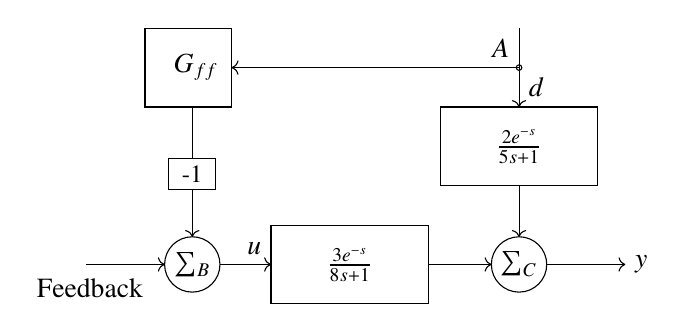
\begin{tikzpicture}
    \draw [->] (-1.35,-5) -- (-0.35, -5); 
    \draw (0,-5) circle (10pt);
    \draw (0,-5) node[]{$\sum_B$};
    \draw [->] (0.35,-5)->(1,-5) node[anchor=south east] {$u$}; 
    \draw (1,-5.5) rectangle (3,-4.5);
    \draw (2, -5) node[] {${\frac{3e^{-s}}{8s+1}}$};
    \draw[->] (3, -5) -- (3.8,-5);
    \draw (4.15,-5) circle (10pt);

    \draw (4.15,-5) node[]{$\sum_C$};
    \draw [->] (4.5, -5) -- (5.5,-5) node[anchor=west] {$y$};
    \draw [->] (4.15,-4) -- (4.15,-4.65);
    \draw [->] (3.15,-3) rectangle (5.15,-4);
    \draw [->] (4.15,-2) -- (4.15,-3) node[anchor= south west] {$d$};
    \draw (4.15, -3.5) node[] {${\frac{2e^{-s}}{5s+1}}$};
    \draw [<-] (0.5,-2.5) -- (4.15,-2.5) node[above left] {$A$};
    \draw (4.15,-2.5) circle (1pt);
    \draw (-0.6, -3) rectangle (0.5, -2);
    \draw (0.05,-2.5) node[] {$G_{ff}$};
    \draw [->] (0,-3) -- (0, -4.65); 
    \filldraw [color=white] (-0.1, -3.65) rectangle (0.1, -4.05);
    \draw (-0.3, -3.65) rectangle (0.3, -4.05);
    \draw (0,-3.85) node[] {\small{-1}};
    \draw (-1.3, -5.3) node[] {Feedback};
\end{tikzpicture}
\hfill(GATE CH 22)\\
\solution 
\iffalse
\let\negmedspace\undefined
\let\negthickspace\undefined
\documentclass[journal,12pt,twocolumn]{IEEEtran}
\usepackage{cite}
\usepackage{amsmath,amssymb,amsfonts,amsthm}
\usepackage{algorithmic}
\usepackage{graphicx}
\usepackage{textcomp}
\usepackage{xcolor}
\usepackage{txfonts}
\usepackage{listings}
\usepackage{enumitem}
\usepackage{mathtools}
\usepackage{gensymb}
\usepackage{comment}
\usepackage[breaklinks=true]{hyperref}
\usepackage{tkz-euclide} 
\usepackage{listings}
\usepackage{gvv}                                        
\def\inputGnumericTable{}                                 
\usepackage[latin1]{inputenc}                                
\usepackage{color}                                            
\usepackage{array}                                            
\usepackage{longtable}                                       
\usepackage{calc}                                             
\usepackage{multirow}                                         
\usepackage{hhline}                                           
\usepackage{ifthen}                                           
\usepackage{lscape}
\usepackage[center]{caption} % center the captions to figure

\newtheorem{theorem}{Theorem}[section]
\newtheorem{problem}{Problem}
\newtheorem{proposition}{Proposition}[section]
\newtheorem{lemma}{Lemma}[section]
\newtheorem{corollary}[theorem]{Corollary}
\newtheorem{example}{Example}[section]
\newtheorem{definition}[problem]{Definition}
\newcommand{\BEQA}{\begin{eqnarray}}
\newcommand{\EEQA}{\end{eqnarray}}
\newcommand{\define}{\stackrel{\triangle}{=}}
\theoremstyle{remark}
\newtheorem{rem}{Remark}
\begin{document}

\newcolumntype{M}[1]{>{\centering\arraybackslash}m{#1}}
\newcolumntype{N}{@{}m{0pt}@{}}

\bibliographystyle{IEEEtran}
\vspace{3cm}

\title{GATE 2022 BM 14 Q} 
\author{ee23btech11223 - Soham Prabhakar More% <-this % stops a space
}
\maketitle
\newpage
\bigskip

\renewcommand{\thefigure}{\theenumi}
\renewcommand{\thetable}{\theenumi}

\bibliographystyle{IEEEtran}

\textbf{Question:} $x\brak{t}$ is a real continuous-time signal whose magnitude frequency response
$\abs{X\brak{j\Omega}}$ is shown below. After sampling $x\brak{t}$ at 100 $rad.s^{-1}$, the spectral point P
is down-converted to \rule{1cm}{0.15mm} $rad.s^{-1}$ in the spectrum of the sampled signal.
\hfill{(GATE 2022 BM 14 Q)}
\begin{figure}[h!]
    \renewcommand\thefigure{1}
    \centering
    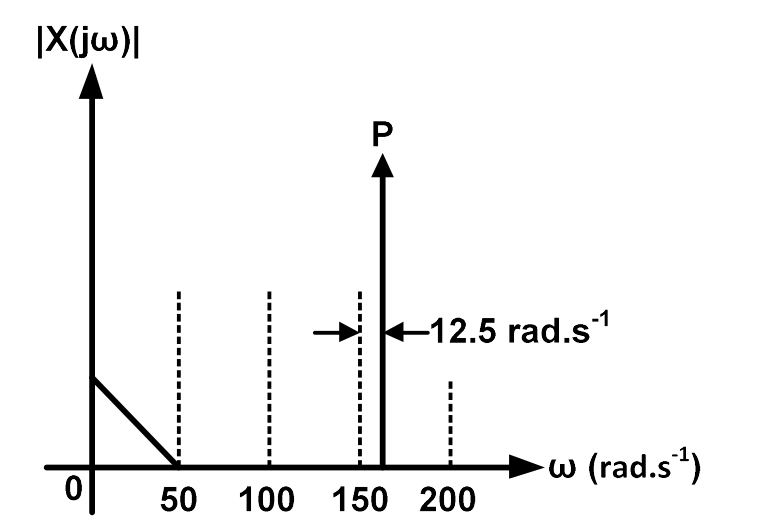
\includegraphics[width=\columnwidth]{2022/BM/14/figs/question.png}
    \caption[short]{Plot of $\abs{X\brak{j\omega}}$}
    \label{fig:2023.bm.14.img1}
\end{figure}

\solution
\fi
\begin{table}[ht]
    \renewcommand\thetable{1}
\begin{tabular}{|c|c|}
    \hline 
    \textbf{Parameter}&\textbf{Description} \\
    \hline
    $w\brak{t}$ & Sampling Function \\
    \hline
	$W\brak{j\omega}$ & Fourier Transform of $w\brak{t}$ \\
    \hline
    $x\brak{t}$ & Input Signal \\
    \hline
    $X\brak{j\omega}$ & Input Signal Frequency Spectrum \\
    \hline
    $x_s\brak{t}$ & Sampled Input Signal \\
    \hline
    $X_s\brak{j\omega}$ & Sampled Signal Frequency Spectrum \\
    \hline
\end{tabular}

\caption{Table of parameters}
\label{Table:1}


\end{table} \\
The sampling function is:
\begin{align}
    w(t) &= \sum_{k = -\infty}^{\infty}\delta\brak{t - \frac{2\pi k}{100}} \\
    W(j\omega) &= 100\sum_{k = -\infty}^{\infty}\delta\brak{j\brak{\omega - 100k}}
\end{align}
then the sampled function: 
\begin{align}
    x_s\brak{t} &= x\brak{t}w\brak{t} \\
    X_s\brak{j\omega} &= X\brak{j\omega} * W\brak{j\omega} \\
    X_s\brak{j\omega} &= \int_{-\infty}^{\infty}X\brak{j\theta}W\brak{j\brak{\omega - \theta}}d\theta \\
    X_s\brak{j\omega} &= 100\sum_{k = -\infty}^{\infty}\int_{-\infty}^{\infty}X\brak{j\theta}\delta\brak{j\brak{\omega - 100k - \theta}}d\theta \\
    X_s\brak{j\omega} &= 100\sum_{k = -\infty}^{\infty}X\brak{j\brak{\omega - 100k}} 
\end{align}
Thus, The down sampled point is at:
\begin{align}
    \omega &= \abs{162.5 - 100k}
\end{align}
where $k$ is the nearest integer to $\frac{162.5}{100}$, which is 2\\
Thus,
\begin{align}
    \omega = 37.5\,rad\,s^{-1}
\end{align}

\begin{figure}[h!]
    \renewcommand\thefigure{2}
    \centering
    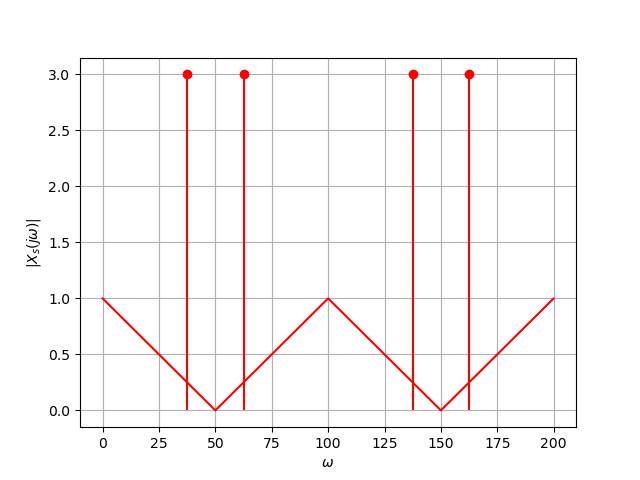
\includegraphics[width=\columnwidth]{2022/BM/14/figs/X_s.png}
    \caption[short]{Plot of $\abs{X_s\brak{j\omega}}$}
    \label{fig:2023.bm.14.img2}
\end{figure}

%\end{document}

\newpage
\item The transfer function of a system is:\\
\begin{center}
$\displaystyle \frac { \brak{s+1}\brak{s+3}}{\brak{s+5}\brak{s+7}\brak{s+9}}$\\
\end{center}
In the state-space representation of the system, the minimum number of state variables (in integer) necessary is\underline{\hspace{1cm}}.\\
\hfill(GATE IN 2022)\\
\solution\\
\iffalse
\let\negmedspace\undefined
\let\negthickspace\undefined
\documentclass[a4,12pt,onecolumn]{IEEEtran}
\usepackage{amsmath,amssymb,amsfonts,amsthm}
\usepackage{algorithmic}
\usepackage{graphicx}
\usepackage{textcomp}
\usepackage{xcolor}
\usepackage{txfonts}
\usepackage{listings}
\usepackage{enumitem}
\usepackage{mathtools}
\usepackage{gensymb}
\usepackage[breaklinks=true]{hyperref}
\usepackage{tkz-euclide}
\usepackage{listings}
\usepackage{circuitikz}
\usepackage{gvv}
\newcommand{\mybmat}[1]{\ensuremath{\begin{bmatrix}#1\end{bmatrix}}}
\begin{document}
\title{
\Huge\textbf{ GATE 2022 Assignment}\\
\Huge\textbf{EE1205} Signals and Systems\\
}
\large\author{Kurre Vinay\\EE23BTECH11036}
\maketitle
\textbf{Question:}
The transfer function of a system is:\\
\begin{center}
$\displaystyle \frac { \brak{s+1}\brak{s+3}}{\brak{s+5}\brak{s+7}\brak{s+9}}$\\
\end{center}
In the state-space representation of the system, the minimum number of state variables (in integer) necessary is\underline{\hspace{1cm}}.\\
\hfill(GATE IN 2022)\\
\solution\\
\fi
\begin{table}[ht!]
\begin{center}
\begin{tabular}{|c|c|c|}
	   \hline
	   variable&value&description\\
	   \hline
	   U\brak{s}&-&input function of the system\\
	   \hline
	   Y\brak{s}&-&output function of the system\\
	   \hline
	   H\brak{s}&$\frac { \brak{s+1}\brak{s+3}}{\brak{s+5}\brak{s+7}\brak{s+9}}$&transfer function of the system.\\
	   \hline
	   I&-&identity matrix \\
	   \hline
	   $\vec{\dot{x}}\brak{t}$ & $A\vec{x}\brak{t} + Bu\brak{t}$&derivative of State function of $ \vec{x}\brak{t}$\\
	   \hline
\end{tabular}
\caption{Table: Input Parameters}
\label{tab:1}
\end{center}
\end{table}
From \tabref{tab:1}
\begin{align}
H\brak{s}&=\frac{\brak{s+1}\brak{s+3}}{\brak{s+5}\brak{s+7}\brak{s+9}}\\
H\brak{s}&= \frac{P}{s+5} +\frac{Q}{s+7} + \frac{R}{s+9}\\
\brak{s+1}\brak{s+3}&=P\brak{s+7}\brak{s+9}+Q\brak{s+5}\brak{s+9}+R\brak{s+5}\brak{s+7} \label{eq:gate2022}
\end{align}
By solving equation \eqref{eq:gate2022} , we get\\
\begin{center}
P = 1\\
Q = -6\\
R = 6
\end{center}

\begin{align}
\implies H\brak{s}&=\frac{1}{s+5} -\frac{6}{s+7} + \frac{6}{s+9}\\
\end{align}
The state-space representation of the system is given by:
\begin{align}
\vec{\dot{x}}\brak{t} &=A\vec{x}\brak{t} + Bu\brak{t}\\
\vec{y}\brak{t} &= C\vec{x}\brak{t} + Du\brak{t}\\
H\brak{s}&=\frac{Y\brak{s}}{U\brak{s}}=C\myvec {sI-A}^{-1}B + D  
\end{align}
Comparing the coefficients:

\begin{align}
A &= \text{coefficient of } s \text{ in } \brak{sI-A}^{-1} \\
B &= \text{coefficient of }  U\brak{s}\\
C &= \text{coefficient of } Y\brak{s} \\
D &= \text{constant term}
\end{align}
 The denominator $\brak{s+5}\brak{s+7}\brak{s+9}$ suggests that the system has three poles. Thus, we'll have a third-order state-space model, and A will be a $3\times 3$matrix.
\begin{align}
\brak{s+5}\brak{s+7}\brak{s+9} &=s^3+21s^2+143s+315\\
A &=  \myvec{0 & 1&0 \\ 0 & 0&1\\-21&-143&-315}\\
\end{align}
A is a $ 3\times 3$ matrix, then the characteristic polynomial will have a degree equal to the size of A, which is $3$.\\
Therefore, the system order, and hence the minimum number of state variables, will be 3.\\

\newpage
\end{enumerate}
